\documentclass[tikz]{standalone}
\RequirePackage{luatex85}
\usepackage{tikz}
\usepackage{tkz-euclide}
\usepackage{tkz-tab}
\usepackage{fourier-otf}
\usepackage{fontspec}

\usetikzlibrary{calc}
\usetikzlibrary{3d}
\usepackage{pgfplots}

\tikzset{
  every picture/.append style={scale=2, every node/.style={scale=2}}
}



\begin{document}
  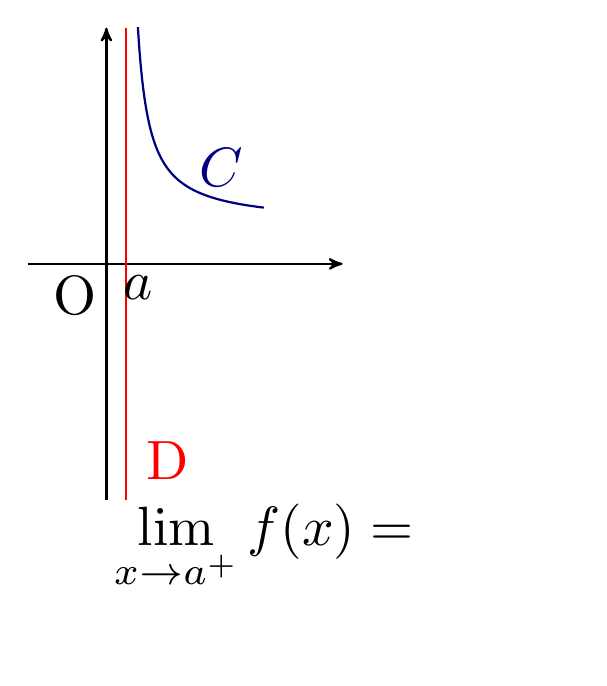
\begin{tikzpicture}[>=stealth', scale=0.5]
\clip (-1,-5) rectangle (6,3);
\draw[->,thick] (-1,0) -- (3,0);
\draw[->,thick] (0,-3) -- (0,3);
\foreach\x in {}
{
\draw[thick] (\x,0.1) -- (\x,-0.1) node[below] {\x};
}
\foreach\y in {}
{
\draw[thick] (0.1,\y) -- (-0.1,\y) node[left] {\y};
}
\draw[thick,blue!50!black] plot[domain=0.26:2,samples=100] (\x,{(2*\x+1)/(4*\x-1)}) node[above left] {$\mathscr{C}$};
\draw[thick,red] (0.25,3) -- (0.25,-3) node[above right] {D};
\node () at (0.4,-0.3) {$a$};
\node () at (-0.4, -0.4) {O};
\node () at (2, -3.6) {$ \displaystyle\lim_{ x \to a^{+}}f(x)=\pinf $};
\end{tikzpicture}
\end{document}
